% 设定文章类型,正文字号为小四,若为五号将-4改为5即可
\documentclass[zihao=-4,UTF8]{report}		

% 导入基本宏包
\usepackage[UTF8]{ctex}       % 设置文档为中文语言(中文paper留此行,删去上一行)
\usepackage{hyperref}   % 宏包:自动生成超链接
\usepackage{amsmath}    % 宏包:数学公式
\usepackage{amssymb}    % 宏包:提供更多数学符号
\usepackage{pifont}     % 宏包:提供了特殊符号和字体

% 文章页面margin设置
\usepackage[a4paper]{geometry}
\geometry{top=1in}
\geometry{bottom=1in}
\geometry{left=0.75in}
\geometry{right=0.75in}   % 设置上下左右页边距
\geometry{marginparwidth=1.75cm}    % 设置边注距离(注释、标记等)

% 页眉页脚设置
\usepackage{fancyhdr}   %宏包:页眉页脚设置
\pagestyle{fancy}
\fancyhf{}
\cfoot{\thepage}
\renewcommand\headrulewidth{1pt}
\renewcommand\footrulewidth{0pt}
\chead{Machanics Notes}    

% 标题自定义设置
\usepackage{titling}  % 宏包:标题设置

% 图片插入自定义设置
\usepackage{graphicx}  % 宏包:图片插入
\usepackage{float}     
\usepackage{caption}\captionsetup[figure]{name=图}  
\usepackage[export]{adjustbox}           

% 文章默认字体设置
\usepackage{fontspec}   % 宏包:更多字体种类
\usepackage{xcolor}    % 宏包:更多颜色设置
\setmainfont{SimSun}    % 设置中文字体为宋体字体
\setmainfont{Times New Roman} % 设置英文字体为Times New Roman

% 参考文献引用设置
\bibliographystyle{unsrt}   % 设置参考文献引用格式为unsrt
\newcommand{\upcite}[1]{\textsuperscript{\cite{#1}}}     % 自定义上角标式引用

% chapter标题自定义设置
\usepackage{titlesec}   
\titleformat{\chapter}[hang]{\normalfont\huge\bfseries\centering}{第\,\thechapter\,章}{20pt}{\Huge}
\titlespacing*{\chapter}{0pt}{-15pt}{20pt} % 控制上方空白的大小
\setcounter{chapter}{-1} % 将chapter序号设置为从零开始

% 文章序言设置
\newcommand{\enabstractname}{Abstract}
\newcommand{\cnabstractname}{序言}
\newenvironment{enabstract}{%
  \par\Large
  \noindent\mbox{}\hfill{\bfseries \enabstractname}\hfill\mbox{}\par
  \vskip 2.5ex}{\par\vskip 2.5ex}
\newenvironment{cnabstract}{%
  \par\Large
  \noindent\mbox{}\hfill{\bfseries \cnabstractname}\hfill\mbox{}\par
  \vskip 2.5ex}{\par\vskip 2.5ex}

% 文档作者信息设置
\title{\textbf{力学笔记\\Machanics Notes}}
\author{丁毅\\ \footnotesize 中国科学院大学,北京 100049\\ Yi Ding \\ \footnotesize University of Chinese Academy of Sciences, Beijing 100049, China}
\date{\footnotesize 2023.12- 2024.1}

 % 开始编辑文章
\begin{document}
\maketitle
\newpage

\addcontentsline{toc}{chapter}{序言} %手动添加为目录
\thispagestyle{fancy}   %显示页码、页眉等
\begin{cnabstract}
{\normalsize 本书是笔者本科时的力学笔记,总结了力学学习中的主要知识,也有适当的拓展延伸。同时,对一些晦涩的物理概念或公式,给出了笔者的个人理解,以帮助读者阅读。}
\end{cnabstract}
\pagenumbering{Roman} %页码为大写罗马数字

\newpage
\addcontentsline{toc}{chapter}{目录}
\tableofcontents
\thispagestyle{fancy}
\newpage
\pagenumbering{arabic} 

\chapter{数学补充}
\thispagestyle{fancy}

\section{数学公式补充}

\chapter{质点运动}
\thispagestyle{fancy}

\section{二维坐标系及其物理量}
\section{其它}

\chapter{牛顿定律与动量定理}
\thispagestyle{fancy}

\section{有关力的知识}
\section{非光滑滑轮问题}
\section{非惯性系与惯性力}
\section{其它}

\chapter{机械能}
\thispagestyle{fancy}

\section{力、功、势能}
\section{碰撞问题}

\chapter{角动量}
\thispagestyle{fancy}

\section{角动量与力矩}
\section{其它}
\section{非惯性质点系中的动力学定理}

\chapter{质心与刚体}
\thispagestyle{fancy}

\section{质心与质点系}
\section{刚体定轴转动}
\section{转动的动力学定理}
\section{刚体平面平行运动}
\section{刚体定点转动}
\section{常见匀质刚体转动惯量}

\chapter{流体}
\thispagestyle{fancy}

\section{流体静力学}
\section{流体动力学}
\section{理想流体的定常流动}
\section{黏性流体的流动}

\chapter{振动与波}
\thispagestyle{fancy}

\section{简谐振动的运动学描述}
\section{简谐振动的动力学性质}
\section{阻尼、受迫、自激振动}
\section{波的运动学描述}
\section{波的干涉}
\section{波的衍射、反射、折射}
\section{波动方程}
\section{波的性质}
\section{电磁波}



\chapter{狭义相对论}
\thispagestyle{fancy}
\section{狭义相对论基本原理}

\subsection{两条基本假设:}
基本假设I(相对性原理):在所有的惯性系中,物理规律都具有相同的形式。\par
基本假设II(光速不变原理):在所有惯性系中,真空光速具有相同量值,与光源运动无关

\subsection{两个重要推论}
设$\beta = \frac{u}{c}$,$u$是物体在$S$系中的速度大小,则有:
\begin{equation*}
  \text{钟慢效应:}t = \frac{t_0}{\sqrt{1-\beta^2}}
  \text{,尺缩效应:}l = l_0\sqrt{1-\beta^2}
\end{equation*}\par
\par
\textcolor{gray}{注:当物体速度方向不平行于长度方向时,可理解为物体沿速度方向的长度按比例缩短。}

\section{洛伦兹变换}
\subsection{线性变换:}
由相对性原理可导出,惯性系之间的时空坐标变换应该是线性的,也即$\left\{\begin{matrix}
  x = a_{11}x'+a_{12}t'\\
  t = a_{21}x'+a_{22}t'
 \end{matrix}\right.$,
 由运动相对性和基本假设II(光速不变原理)解出四个待定的系数,即可得到洛伦兹变换。

\subsection{Lorentz Transformations:}
由8.2.1的思路,解出四个待定的系数,得到Lorentz Transformations:
\begin{align*}
   &\text{正变换:}
   \textcolor{red}{x=\frac{x'+vt'}{\sqrt{1-\beta ^2}}},\;\;
   \textcolor{red}{y=y'},\;\;
   \textcolor{red}{z=z'},\;\;
   \textcolor{red}{t=\frac{t'+\frac{vx'}{c^2}}{\sqrt{1-\beta ^2}}}\\
   &\text{逆变换:}
    x'=\frac{x-vt}{\sqrt{1-\beta ^2}},\;\;
    y=y',\;\;
    z=z',\;\;
    t'=\frac{t-\frac{vx}{c^2}}{\sqrt{1-\beta ^2}}
\end{align*}


\subsection{两个限定条件:}
光是物质,它的真空速度为$c$,但光不是物体,不可取为参考物,不可构成度量其他物体运动的参考系。\par
为使狭义相对论符合因果律的要求,任一惯性参考系中,物体的速度大小不可超过$c$。
\subsection{本征时间:}
任何一个动力学系统测量自身物理过程所经历的时间间隔,是指用一个相对它静止的时钟(在此参考系下速度为$0$)测得的时间间隔,这样测得的时间间隔称为本征时间。
\subsection{相对论尺度下的多普勒效应:}
如图\ref*{图:多普勒效应},点B为接收点,点P为光源,P相对于B的速度$v$与PB的夹角为$\phi$,则有结论:


\begin{figure}[h]
  \centering
  \begin{minipage}[c]{0.7\textwidth}
    \begin{align*}
      &\phi = 0\text{,P朝向B运动:}\nu=\nu_0\sqrt{\frac{1+\beta}{1-\beta}}> \nu_0\text{,蓝移}\\
      &\phi = \pi\text{,P背离B运动:}\nu=\nu_0\sqrt{\frac{1-\beta}{1+\beta}}< \nu_0\text{,红移}\\
      &\phi = \pm \frac{\pi}{2}\text{,P作横向运动:}\nu=\nu_0\sqrt{1-\beta^2}< \nu_0\text{,红移}
    \end{align*}
  \end{minipage}%
  \begin{minipage}[]{0.2\textwidth}
    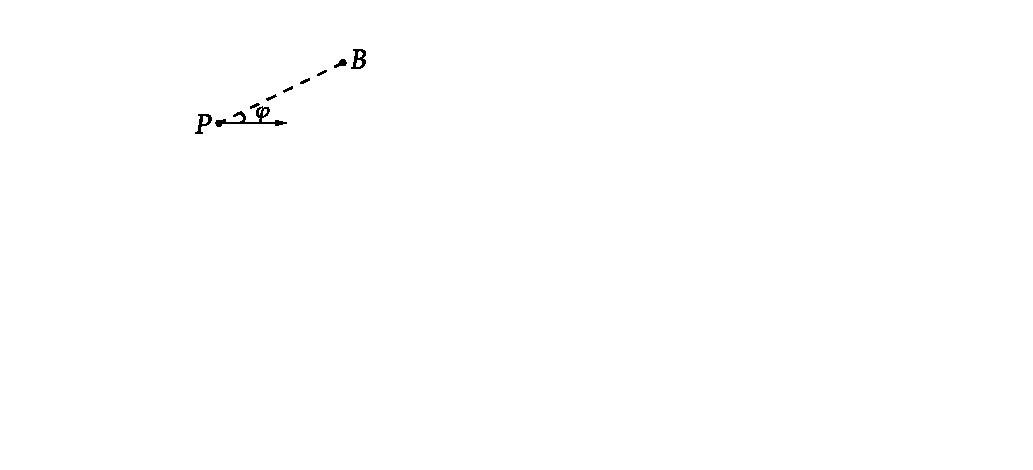
\includegraphics[width=\linewidth]{pic/多普勒效应 (2).pdf}
    \caption{}
    \label{图:多普勒效应}
  \end{minipage}
\end{figure}

\subsection{速度变换:}
设S'系相对S系的速度为$v$(沿$x$轴),物体P在S'系中的速度为$\vec{u}'$,则有:
\begin{align*}
  &u_x=\frac{u_x'+v}{1+\frac{vu_x'}{c^2}},\;\;u_y=\frac{\sqrt{1-\beta^2}}{1+\frac{vu_{\textcolor{red}{x}}'}{c^2}}\cdot u_y',\;\;u_z=\frac{\sqrt{1-\beta^2}}{1+\frac{vu_{\textcolor{red}{x}}'}{c^2}}\cdot u_z'\text{,逆变换即为:}\\
  &u_x'=\frac{u_x-v}{1+\frac{vu_x}{c^2}},\;\;u_y'=\frac{\sqrt{1-\beta^2}}{1+\frac{vu_{\textcolor{red}{x}}}{c^2}}\cdot u_y,\;\;u_z'=\frac{\sqrt{1-\beta^2}}{1+\frac{vu_{\textcolor{red}{x}}}{c^2}}\cdot u_z\text{,并且有:}\\
  &\left | \vec{u} \right |^2=c^2-\frac{(1-\beta^2)\left | \vec{u}' \right |^2}{(1+\frac{vu_x'}{c^2})^2} \text{,由此推出:}\left | \vec{u} \right |^2<c^2\Longleftrightarrow\left | \vec{u}' \right |^2<c^2
\end{align*}

\subsection{加速度变换:}
需要说明的是,加速度的变换与速度有关,因此牛顿定律不再普遍成立。
\begin{align*}
  &a_x=\frac{(1-\beta^2)^{\frac{3}{2}}}{(1+\frac{vu_x'}{c^2})^3}\cdot a_x'\\
  &a_y=\frac{1-\beta^2}{(1+\frac{vu_x'}{c^2})^2}\cdot a_y'-\frac{(1-\beta^2)\frac{vu_y'}{c^2}}{(1+\frac{vu_x'}{c^2})^3}\\
  &a_z=\frac{1-\beta^2}{(1+\frac{vu_x'}{c^2})^2}\cdot a_z'-\frac{(1-\beta^2)\frac{vu_z'}{c^2}}{(1+\frac{vu_x'}{c^2})^3}
\end{align*}

\section{相对论动力学}

\subsection{受力变换:}
参考系的转换会使得物体受力发生变化:
\begin{equation*}
  F_x=\frac{F_x'+\frac{v}{c^2}(\vec{u}\cdot \vec{F})}{1+\frac{vu_x'}{c^2}},\;\;
  F_y = \frac{\sqrt{1-\beta^2}}{1+\frac{vu_x'}{c^2}}\cdot F_y',\;\;
  F_z = \frac{\sqrt{1-\beta^2}}{1+\frac{vu_x'}{c^2}}\cdot F_z'
\end{equation*}

\subsection{牛顿定律修正:}
转换参考系时,不仅需要根据8.3.1完成受力变换,还需要使用修正后的牛顿定律:
\begin{align*}
  &\text{牛顿第I定律:仍成立。}\\
  &\text{牛顿第II定律:改用动量..形式}\;\vec{F}=\frac{\mathrm{d} (m\vec{v})  }{\mathrm{d} t}\text{,其中$m$为动质量。}\\
  &\text{牛顿第III定律:不再普遍成立,改用动量守恒。}
\end{align*}

\subsection{动量、能量变换:}
转换参考系时,动量和能量也需要进行变换:
\begin{equation*}
  p_x=\frac{p_x'+\frac{vE'}{c^2}}{\sqrt{1-\beta^2}},\;\;p_y=p_y',\;\;p_z=p_z',\;\;E=\frac{E'+vp_x'}{\sqrt{1-\beta^2}}
\end{equation*}

\subsection{质量变换、能量分解:}
转换参考系时,静质量不变,但动质量和动能都改变:
\begin{align*}
  &m=\frac{1+\frac{vu_x'}{c^2}}{\sqrt{1-\beta^2}},\;\;\beta = \frac{v}{c}\Longrightarrow \textcolor{red}{m=\frac{m_0}{\sqrt{1-\beta^2}}},\;\;\beta = \frac{u}{c}\text{,$m_0$称为静质量,$m$称为动质量}\\
  &E=E_k+E_0,\;\;E=mc^2,\;\;E_0=m_0c^2\Longrightarrow E_k = mc^2-m_0c^2\text{,$E_k$称为动能}
\end{align*}

\subsection{能量动量方程:}
任一惯性参考系中,都满足如下方程:
\begin{align*}
  \textcolor{red}{mc^2}&\textcolor{red}{=(pc)^2+m_0c^2}\\
  E^2&=(pc)^2+E_0^2
\end{align*}

\section{第八章思考题}

\noindent\textbf{1. 在相对论尺度下,伽利略速度分解(运动的合成与分解)是否仍然适用,如果不是,那该如何进行运动的分解与合成?}\par
下面给出一个例子, 试探究其是否正确,如果不正确,错误在哪里?\par
$S$系中有一静止时各边长为$a$的正方形面板,如图\ref{静止正方形}所示。今使面板沿其对角线方向匀速运动,速度大小为$v$。某学生将$v$沿静止时的两条直角边方向分解,每一个方向上的分速度大小均为$v'=\frac{v}{\sqrt{2}}$。考虑到每一直角边的长度收缩,他认为$S$系中运动面板的形状将如图\ref{速度分解图}所示,是一个边长为$a'=\sqrt{1-\frac{v'^2}{c^2}}\cdot a$的正方形。

\begin{minipage}[b]{0.45\columnwidth}
  \begin{figure}[H]
    \centering
    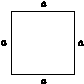
\includegraphics[scale=3]{pic/静止正方形.pdf}
    \caption{静止的正方形}
    \label{静止正方形}
  \end{figure}
\end{minipage}%
\begin{minipage}[b]{0.45\columnwidth}
    \begin{figure}[H]
      \centering
      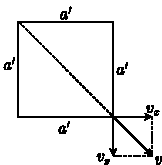
\includegraphics[scale=1.6]{pic/速度分解图.pdf}			
      \caption{速度分解}
      \label{速度分解图}
    \end{figure}
\end{minipage}

\noindent\textbf{2. 长度收缩的适用条件?}\par
下面给出一个例子,试解释长度收缩在这里出现的问题。\par
惯性系$S$中有一柄剑和一个桶(都为刚体),剑长和桶深相同,如图\ref{剑与桶}桶在$S$系中静止,剑相对桶的运动速度为$v$,问剑先刺到桶还是剑柄先被桶挡住?从长度收缩的角度可得,在剑参考系中,桶收缩,剑先刺到桶,在桶参考系中,剑收缩,剑先被挡住,两者相互矛盾。而正确的结论是,在两个参考系中,剑刺到桶和剑被挡住两个事件都是同时发生,试加以解释论证。
\begin{figure}[H]
  \centering
  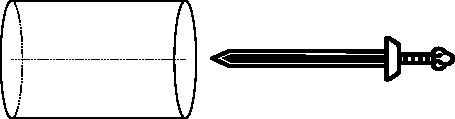
\includegraphics[scale=1.5]{pic/剑与桶.pdf}		
  \caption{剑与桶}
  \label{剑与桶}
\end{figure}

\end{document}

